\scanpage{12}\mspage{11}
Il serait \unsure{donc} intéressant de dégager les axiomes pertinents des ateliers spacieux ou polyédraux, en termes cette fois de $(\unsure{M|\mathcal{M}},\leq,\ll,\parallel)$ -- en laissant de côté la donnée de $\widetilde{\mathcal{F}}$ (ce qui est licite dans le cas des \inserted{ateliers} figures de type fini \unsure{...}\deleted{\unsure{)}}, et dans le cas général la donnée de $\widetilde{\mathcal{F}}$ se réduit à celle de \unsure{certaines|certains} \unsure{antifiltres} -- i.e. d'une notion de familles \uline{\unsure{loc|loc.} \unsure{finies|finie}} de \unsure{strates|str.}\unsure{...})

\deleted{Dans le cas des ateliers spacieux, on a}

\deleted{\uline{Axiomes} \uline{\unsure{des|de} \unsure{supports|support|propreté}}}

\deleted{\uline{\unsure{At S$_0$|At P$_0$}} On voudrait que le}

Je tombe sur un bec \deleted{\unsure{sérieux|délicat}}\inserted{ennuyeux}, dans le formalisme $\ll$ dans le cas d'un atelier simplicial \inserted{(plus \unsure{génlt|gén.}, \unsure{polyédral})}. ai admis que $\ll$ entre simplexes (d'un espace topologique, ou modéré, disons) était la relation $\ll$ des figures \uline{ensemblistes}, de sorte que j'ai accepté l'inclusion d'un $\Delta^1$ \unsure{ds|dans} un $\Delta^2$
\figure{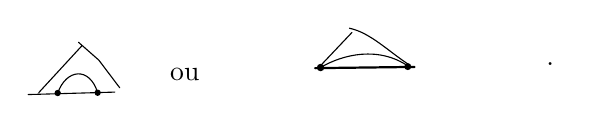
\begin{tikzpicture}[x=.78cm,y=.78cm,line cap=round,line join=round]
\draw (-.10,0)--(1.31,.04) (.07,.03)--(.77,.79) (.72,.85)--(1.05,.56)--(1.39,.11);
\draw (.38,.025) .. controls (.52,.42) and (.90,.46) .. (1.03,.03);
\fill (.38,.025) circle (.052) (1.03,.03) circle (.052);
\node at (2.45,.33) {ou};
\begin{scope}[shift={(4.66,.44)}]
\draw (-.03,0)--(.51,.57) (.47,.64) .. controls (.81,.57) and (1.12,.25) .. (1.45,.04);
\draw[line width=.8pt] (-.09,-.01)--(1.53,.01);
\draw (0,0) .. controls (.37,.22) and (.95,.35) .. (1.43,.02);
\fill (0,0) circle (.061) (1.42,.015) circle (.057);
\end{scope}
\node at (8.40,.49) {.};
\end{tikzpicture}}
ce qui me conduit à accepter des subdivisions de $\Delta^2$ en deux triangles comme ceci
\figure{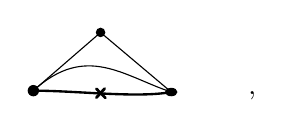
\begin{tikzpicture}[x=.88cm,y=.88cm,line cap=round,line join=round]
\draw (0,0)--(.97,.84)--(1.99,-.02);
\draw[line width=.85pt] (0,0) .. controls (.63,.00) and (1.50,-.11) .. (1.99,-.02);
\draw (0,0) .. controls (.76,.69) and (1.30,.21) .. (1.99,-.02);
\fill (0,0) circle (.082) (.97,.84) circle (.069) (1.99,-.02) ellipse (.09 and .061);
\draw[line width=1pt] (.91,.026)--(1.04,-.105) (.91,-.10)--(1.03,.031);
\node at (3.16,-.07) {,};
\end{tikzpicture}}
ce que personne ne \unsure{regardera} comme une subdivision simpliciale ! C'est le modèle des \uline{simplexes affines} dans un espace affine qui a guidé les gens, et il faut \unsure{utiliser}
